\section{Aufbau und Durchführung}
\label{sec:Durchführung}
\subsection{Aufbau}
Die Wärmeleitfähigkeit lässt sich mit dem Aufbau nach Abbildung \ref{abb:aufbau}
bestimmen. Auf einer Platte befinden sich vier unterschiedlich große,
rechteckige Probestäbe, zwei davon sind aus Edelstahl und jeweils einer
aus Messing und Aluminium. Diese werden von einem Peltierelement simultan
geheizt oder gekühlt. Mit Thermoelementen werden Temperaturen an acht Messstellen
gemessen und mittels Datenlogger "Xplorer GLX" gespeichert.
\begin{figure}
  \centering
  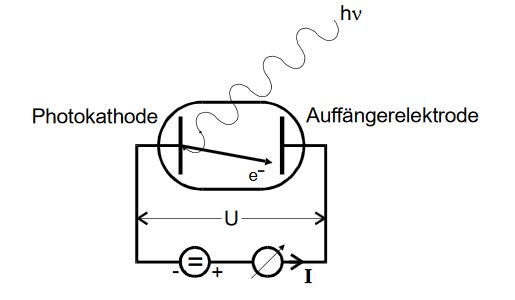
\includegraphics[width=0.7\textwidth]{aufbau.png}
\caption{Versuchsaufbau.\cite{sample}}
\label{abb:Aufbau}
\end{figure}
\subsection{Statische Methode}
Zu Begin wird die Abtastrate des GLX auf $5 \si{\second}$ gestellt.
Bei maximalem Strom werden $8 \si{\volt}$ Betriebsspannung für das
Peltierelement eingestellt.Die Apparatur wird mit Isolierung aufgeheizt.
Die Messung wird solange durchgeführt bis an Thermoelement $T_7$ eine
Temperatur von $45\si{\degreeCelsius}$ erreicht wird.
Anschließend wird die Apparatur gekühlt.
\subsection{Dynamische Methode}
In dieser Messung wird die Abtastrate auf $2\si{\second}$
und die Betriebsspannung auf $10,5\si{\volt}$ gesetzt.
Alle $40\si{\second}$ werden die Stäbe aufgeheizt bzw. gekühlt.
Für 10 Perioden werden die Temperaturen erfasst.
Anschließend werden die Stäbe runtergekühlt.
Dieser Vorgang wird für eine Periode von $200\si{\second}$ wiederholt.
Dementsprechend wird wieder $100\si{\second}$ geheizt und $100\si{\second}$ gekühlt.
